\section{Продолжение строк. Алгоритм Ахо -- Корасик для нахождения всех вхождений набора подстрок.}%
Мы хотим научиться искать все вхождения строк из набора в некотором тексте.

\subsection{Построение бора.}%
\begin{Def}
	\textbf{Бор} --- дерево, в котором каждая вершина обозначает строку, а каждое ребро обозначает букву. Строка, соответствующая вершине (то есть заканчивающаяся в этой вершине), получается конкатенацией всех букв, соответствующих ребрам пути из корня в эту самую вершину. По определению, корню бора соответствует пустая строка.
\end{Def}

\begin{Def}
	\textbf{Терминальная вершина} бора для набора слов --- вершина, которой соответствует слово из этого набора.
\end{Def}


Для добавления строки в бор мы: \\
Прочитав очередной символ в цикле по строке, переходим по соответствующему ему ребру или создаем такое ребро если потребуется. \\
После завершения строки помечаем последнюю вершину как терминальную.

Таким образом, бор строится за линейное по сумме всех строк в наборе время.

\subsection{Преобразование бора в автомат.}%
Будем понимать вершины бора и соответствующие им строки как состояния конечного детерминированного автомата. Однако мы сталкиваемся с проблемой, ребер бора не достаточно для отражения всех возможных переходов между состояниями автомата. 
\begin{example}
	Ребра бора не отражают тот факт, что перейдя под воздействием символов $"ad"$ в некоторое состояние  $S_1$ мы все еще можем перейти в состояние  $S_2$.
    \begin{center}
        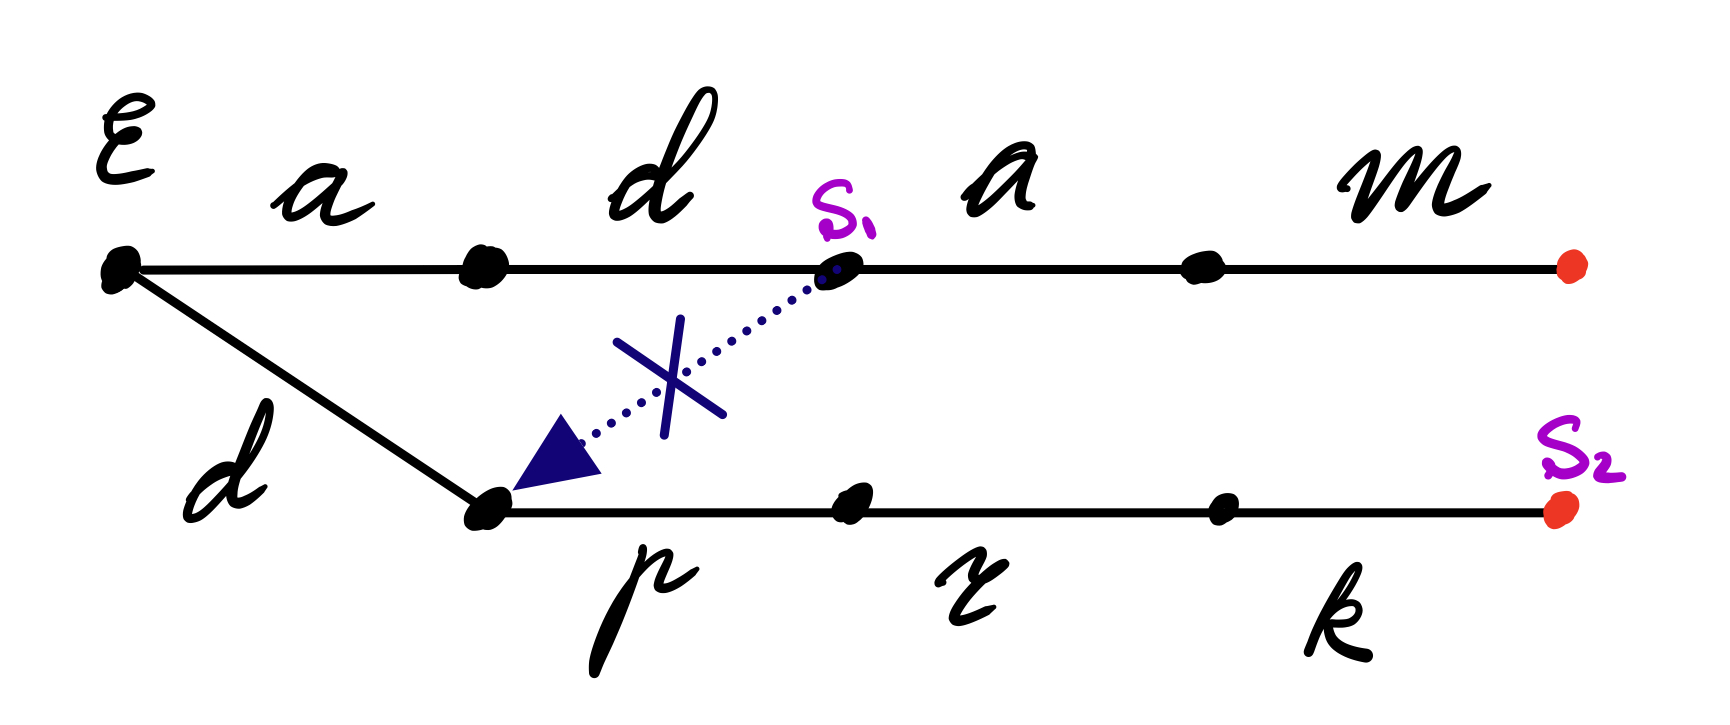
\includegraphics[scale = 0.2]{images/lect06/adam_dprk.jpeg}
    \end{center}
\end{example}

\begin{Def}
	\textbf{Суффиксная ссылка} вершины $v$ --- ссылка (мнимая стрелка в боре) на вершину $u$, такую, что состояние $u$ --- наибольший собственный суффикс состояния $v$, а если такой вершины  $u$ нет, то ссылка на корень. По определению, ссылка из корня ведет в корень.
\end{Def}

\begin{example}
	Для бора строк $"adam"$ и $"dprk"$ единственной суффиксной ссылкой, не ведущей в корень, будет ссылка из состояния $"ad"$, в состояние $"d"$, зачеркнутая на рисунке выше.
\end{example}

\subsubsection{Нахождение суффиксных ссылок.}

\textbf{Чтобы найти суффиксную ссылку} для вершины $v$:  \\
Если $v$ -- корень, то и его суффиксная ссылка тоже корень.
В противном случае: \\
\begin{itemize}
\item Пусть $c$ --- буква, преводящая из родителя в вершину $v$. 
\item Рассмотрим в качестве текущей вершины суффиксную ссылку родителя. 
\item Пока в рассматриваемой вершине нет ребра, соответствующего букве $c$, будем прыгать дальше, рассматривая ее суффиксную ссылку. 
\item Если мы уперлись в корень, то корень и является суффиксной ссылкой вершины $v$. 
\item Если мы нашли вершину $u$, с ребром  $c$, то суффиксной ссылкой будет вершина, в которую ребро  $c$ переводит  вершину $u$.
\end{itemize}

Концептуально, мы берем наибольший собственный суффикс родителя и откусываем от него по одной букве слева, пока не получится подстрока, которая добавлением одного символа становится собственным суффиксом нашей исходной строки.

\begin{lstlisting}[language = C++]
    auto get_suflink(Node_t* node){
        
        if (node == root) return root;

        auto last_c = node->c;
        auto parent = node->parent;

        while(parent != root && parent->go[last_c] == nullptr){
            parent = get_suflink(parent);
        }

        if (parent == root) return root;
        return parent->go[last_c];
    }
\end{lstlisting}

Этот алгоритм терминируется, ведь на каждом шаге мы поднимаемся выше по бору, а значит рано или поздно дойдем до корня.

Мы считаем суффиксные ссылки рекурсивно, но этот процесс можно \textbf{оптимизировать, записав суффиксную ссылку в вершину}, ведь после построения автомата она меняться не будет.
Тогда мы можем ввести универсальную автоматную функцию перехода, которая не делает различия между суффиксными ссылками.

$jump(node, c) = $
\begin{itemize}
    \item[$\textperiodcentered$] $son\_c$, \text{если ребро бора $c$ переводит вершину $node$ в  $son\_c$}
    \item[$\textperiodcentered$] $null$, \text{если $node$ --- корень, у которого нет ребра бора $c$}
    \item[$\textperiodcentered$] $go(suflink(node), c)$, \text{иначе}
\end{itemize}

С учетом концепции универсальности перехода, переход по суффиксной ссылке вершины --- переход из суффиксной ссылки родителя по ребру $c$, где  $c$ --- ребро, которое перевело родителя в вершину.
\begin{lstlisting}[language = C++]
    suflink(node) = jump(suflink(node->parent), node->c); 
\end{lstlisting}

Тогда чтобы посчитать суффиксные ссылки мы пойдем по дереву по слоям, высчитывая suflink и jump одновременно:
\begin{enumerate}
    \item Для корня все известно.
    \item Для первого слоя suflink ведет в корень, а jump вниз или по suflink в корень и по go от него.
    \item Для каждого из следующих уровней мы можем найти и suflink и jump за $O(1)$, ведь для родителя, который находится уровнем выше мы уже все посчитали.
\end{enumerate}
Концептуально это BFS.

\subsection{Поиск вхождений при помощи автомата.}
Для поиска набора строк в тексте:
\begin{enumerate}
    \item Построим автомат по набору строк. 
    \item Каждый раз будем считывать букву текста, и совершать переход по ней в автомате.
\end{enumerate}
При этом, мы поймем, что нашли совпадение строки из набора, если текущая вершина терминальная, \textit{а также если, двигаясь по суффиксным ссылкам, мы можем достигнуть терминальной вершины.} \\
Из-за этого отягчающего обстоятельства, определение вхождения строки в текст для каждого состояния будет занимать линейное время.
Оптимизируем это движение по суффиксным ссылкам.

\subsection{Нахождение сжатых терминальных ссылок.}
\begin{Def}
    \textbf{Сжатая терминальная ссылка} вершины $v$ --- ближайшая достижимая по суффиксным ссылкам из $v$ вершина$w$, являющаяся терминальной и не совпадающая с $v$.
\end{Def}

\begin{example} 

Сжатые терминальные ссылки отмечены синим.
\begin{center}
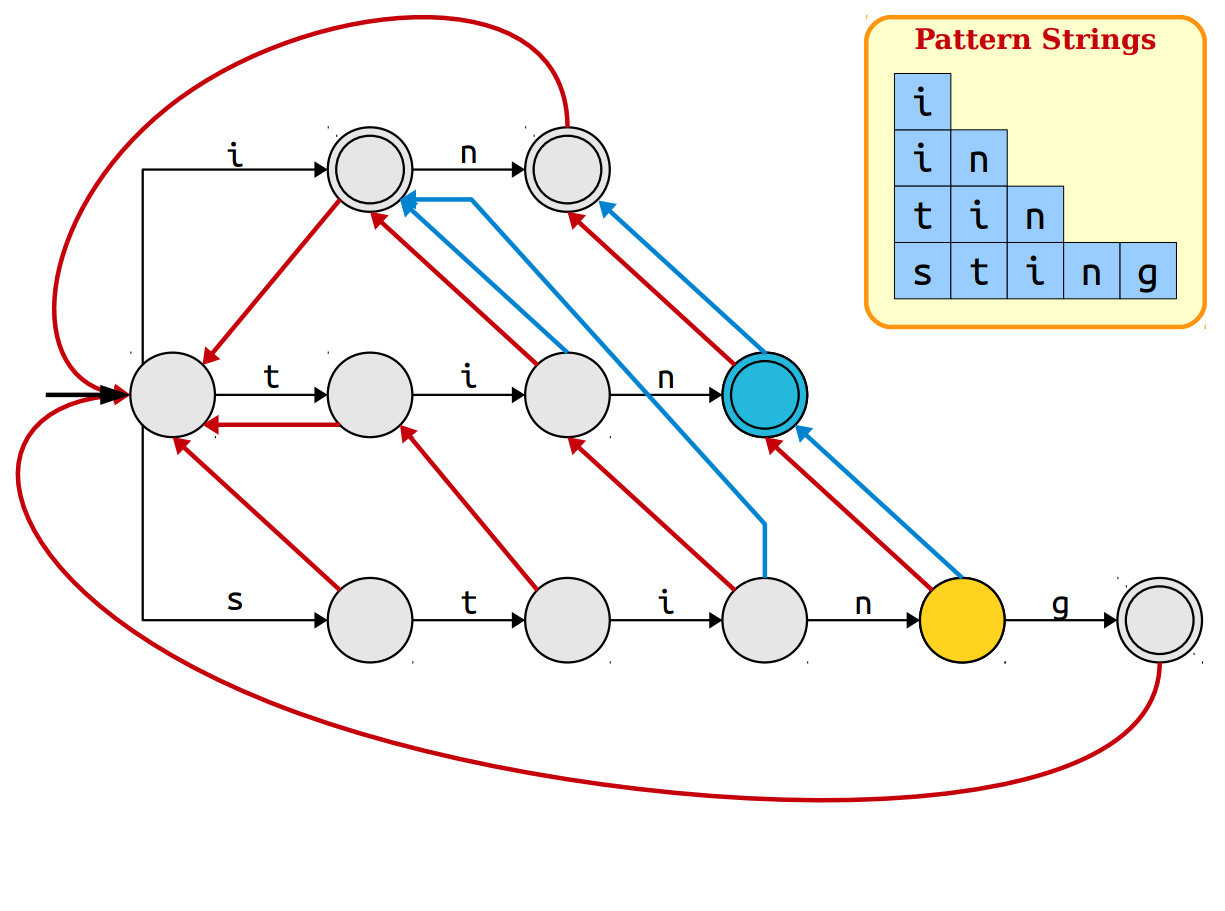
\includegraphics[scale = 0.3]{"images/lect06/Aho-Corasick-complete-links.png"}
\end{center}
\end{example}

Концептуально, сжатые терминальные ссылки собирают в односвязный список все терминальные вершины, а значит и все подстроки, вхождение которых имело место при достижении текущего состояния.
Таким образом, учитывая что сжатая терминальная ссылка ведет только наверх, мы сможем построить эти ссылки по слоям при помощи BFS.
\newpage
\begin{lstlisting}[language = C++]
    if (suflink(node)->is_terminal){
        complete_link(node) = suflink(node);
    }

    else {
        complete_link(node) = complete_link(suflink(node));
    }
\end{lstlisting}

\subsection{Алгоритм с использованием сжатых терминальных ссылок.}
\begin{enumerate}
    \item Построим автомат по набору строк.
    \item Построим сжатые терминальные ссылки в автомате.
    \item Для каждого считанного символа $c$:
        \begin{enumerate}
            \item $cur\_node = go(root, c)$
            \item Если $cur\_node == null$, вхождение соответствует, идем дальше.
            \item В противном случае, засвидетельствуем вхождение подстроки, соответствующей текущей вершине, если она терминальная, а также всех ее сжатых терминальных ссылок.
        \end{enumerate}
\end{enumerate}

\subsection{Сложность алгоритма.}
Пусть $\Sigma$ --- суммарная длина подстрок в наборе,  $T$ --- длина текста, по которому осуществляется поиск, $Ans$ --- число найденных вхождений.

\begin{enumerate}
    \item Построение бора требует $O(\Sigma)$
    \item Построение суффиксных ссылок, по сути, BFS по дереву, требует  $O(\Sigma)$
    \item Построение сжатых терминальных ссылок, также BFS по дереву, требует $O(\Sigma)$
    \item Цикл по каждому из символом --- $O(T)$
    \item Проходы по сжатым терминальным ссылкам суммарно займут  $O(Ans)$
\end{enumerate}

Итого, имеем $O(\Sigma + T + Ans)$
